%!TEX TS-program = xelatex 
%!TEX encoding = UTF-8 Unicode 

\documentclass[fontsize=11pt, paper=a4, 
  DIV15,
  normalheadings,
  parskip=half-, 
  pointlessnumbers]{scrartcl}

\usepackage[british]{babel} 

\usepackage{fontspec,xltxtra,xunicode} 
\defaultfontfeatures{Mapping=tex-text} 

\setromanfont[Mapping=tex-text]{DejaVu Serif}
\setsansfont[Scale=MatchLowercase,Mapping=tex-text]{Helvetica} 
\setmonofont[Scale=1.0]{Courier New} 

\frenchspacing

\usepackage{graphicx}
\graphicspath{{../../bilder/}}
\graphicspath{{./bilder/}}

\usepackage{longtable}

\usepackage{philokalia}

%%%

%!TEX TS-program = xelatex
%!TEX encoding = UTF-8 Unicode

\usepackage{xspace} \xspaceaddexceptions{”}
\usepackage{ifthen}

\newcommand{\ch}[1]		{chapter~\ref{#1}}
\newcommand{\sect}[1]		{section~\ref{#1}}
\newcommand{\fig}[1]		{figure~\vref{#1}}
\newcommand{\Fig}[1]		{Figure~\vref{#1}}
\newcommand{\tbl}[1]		{table~\vref{#1}}

\newcommand{\ie}			{i.e. }
\newcommand{\eg}			{e.g. }

\newcommand{\qq}			{\qquad}

\newcommand{\spitz}[1]		{\ensuremath{\langle}#1\ensuremath{\rangle}}

\newcommand{\mehrzeilen}[1][1]{\enlargethispage{#1\baselineskip}}


% Zeilenabstand

\usepackage{setspace}
\newenvironment{enum}{\begin{enumerate} \singlespacing} {\end{enumerate}}
\newenvironment{items}{\begin{itemize} \singlespacing} {\end{itemize}}


% verbatim

\usepackage{verbatim}

\usepackage{alltt}
\newcommand{\klein}{\small}
\newenvironment{exakt}[1][\small]{\singlespacing#1\begin{alltt}}{\end{alltt}}

\usepackage{shortvrb}
\MakeShortVerb{\§}


%%%%%%%%%%%%%%%%%%%%%%%%%%%%%%%%

% xml commands
% use for any xml markup, brackets supplied
\newcommand{\xml}[1]{§<#1>§}
% use for milestone tags
\newcommand{\xms}[1]{§<#1/>§}
% closing element markup
\newcommand{\xmcl}[1]{§</#1>§}
% full xml markup example
\newcommand{\xmex}[1]{§#1§}
% attribute markup, the first argument is the element name
\newcommand{\attr}[2]{§@#2§}

\newcommand{\bold}{\textbf}
% ligature
\newcommand{\li}[1]{\bold{\{}#1\bold{\}}}

\newcommand{\xs}{\scriptsize}
\newcommand{\s}{\footnotesize}

%

\newcommand{\bs}{\textbackslash}
\newcommand{\tld}{\textasciitilde}

\newcommand{\tocspace}{\addtocontents{toc}{\protect\vspace{1mm}}}

\newcommand{\unicode}[1]{{\fontspec{Apple Symbols}{\Large #1}}}
\newcommand{\§}{{\char"00A7}}

%%%%%%%%%%%%%%%%

\newcommand{\htsc}[1]{\emph{#1}}
\newcommand{\lig}[1]{\fontspec{Hoefler Text}{\Large #1}}
\newcommand{\fraktur}[1]{{\fontspec{BreitkopfFraktur}{\LARGE #1}}}

%

\newenvironment{mainrule}{}{}
\newenvironment{mainruleLessImportant}{}{}
\newenvironment{clarification}{\s}{}
\newenvironment{exception}{\htsc{Exception:}}{}
\newenvironment{note}{\textbf{Please note:}}{}
\newenvironment{crossref}{\s\ensuremath{\longrightarrow}}{}

%

\newenvironment{sampleImage}[2][]{\parbox{\linewidth}{{\htsc{Example#1}} \\[3mm] \includegraphics[width=\linewidth]{#2}}}{}
\newenvironment{sampleImageSmall}[3][]{\parbox{\linewidth}{{\htsc{Example#1}} \\[3mm] \includegraphics[#2]{#3}}}{}

\newenvironment{example}[1][]{\htsc{Example#1} \\}{}
\newenvironment{exampleTest}[2][]{\parbox{\linewidth}{\htsc{Example #1} \\[3mm] #2}}{} % ??

\newenvironment{liste}[1][]{\htsc{List#1} \\}{}
\newenvironment{tabelle}[1][]{\htsc{Table#1} \\}{}

%

\newenvironment{typeLatin}{\begin{alltt}\s\begin{tabular}{@{}l}}{\end{tabular}\end{alltt}}

\newfontfamily{\greek}[Scale=0.95]{Courier New}
\newenvironment{typeGreek}{\begin{alltt}\greek\s\begin{tabular}{@{}l}}{\end{tabular}\end{alltt}}

\newenvironment{typeMath}{\begin{alltt}\begin{tabular}{l}}{\end{tabular}\end{alltt}}

%

\newfontfamily{\muh}[Scale=0.9]{DejaVu Serif}
\newcommand{\someText}{...} % {{\muh\textit{(some text)}}}
\newcommand{\untranscribedText}{...} % {{\muh\textit{(some untranscribed text)}}}
\newcommand{\notTranscribed}{{\muh\textit{(not transcribed)}}}
\newcommand{\missingText}[1]{{\muh\textit{(#1)}}}

%% Chinese bits
\newenvironment{typeChinese}{\begin{alltt}\s\begin{tabular}{@{}l}}{\end{tabular}\end{alltt}}

\newcommand{\chin}[1]{{\fontspec{Sun-ExtA}{#1}}}
\newcommand{\sunExtA}[1]{{\fontspec{Sun-ExtA}{#1}}}
\newcommand{\sunExtB}[1]{{\fontspec{Sun-ExtB}{#1}}}

\newcommand{\mincho}[1]{{\fontspec{MS Mincho}{#1}}}
\newcommand{\hira}[1]{{\fontspec{HiraMinPro-W3}{#1}}}

\newcommand{\f}[1]{\bold{#1}} % f für fett
\newcommand{\z}[1]{\chin{#1}} % z für Zeichen


\begin{document}

\begin{center}
  {\fontspec{Helvetica}{\LARGE \textbf{
        Special Instructions for "Ben Cao Jing Ji Zhu (\chin{本草經集注})”
        \\[3mm]
        (Addendum to Data Entry Specs for Chinese Text 2.1) 
  }}} \\[5mm]
  \large Klaus Thoden, Shih-Pei Chen, Georg Freise

  \normalsize Max Planck Institute for the History of Science, Berlin, Germany

  \today
\end{center}

\section{Footnote marks}
\begin{mainrule}
  This book contains footnotes with anchors in the main text. The
  footnote marks in the main text are surrounded by Chinese
  parentheses. Please tag them with §<a>§ and §</a>§.
\end{mainrule}

%% \begin{clarification}
%% Type the §<tf>§ and §</tf>§ tags on separate lines. On each page, type the first text flow before the second text flow.
%% \end{clarification}
\vspace{3mm}
%%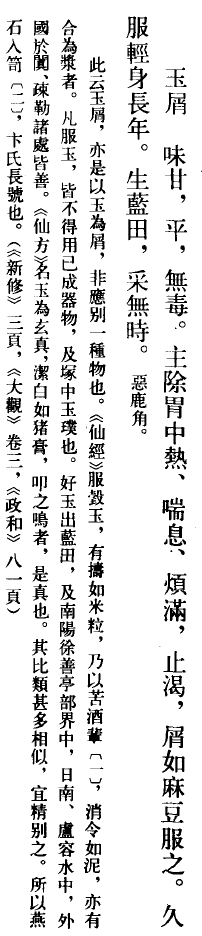
\includegraphics[height=4cm]{image1}
\begin{sampleImageSmall}[\ 1: \, Footnote marks.]{height=10cm}{image1.png}
\end{sampleImageSmall}
%% \begin{tabular}{@{}ll}
%%   \parbox[b]{131mm}{
\begin{typeChinese}
  \f{<h3>}\z{玉屑}\f{</h3>}\\
  \f{<p>}\z{味甘,平,無毒。主除胃中熱、喘息、煩滿,止渴,屑如麻豆服之。久}\\
  \z{服輕身長年。生藍田,采無時。}\f{<sm>}\z{惡鹿角。}\f{</sm></p>}\\
  \f{<p><sm>}\z{此云玉屑,亦是以玉為屑,非應別一種物也。《仙經》服榖玉,有擣如米粒,乃以苦酒輩}\f{<a>}\z{﹝一﹞}\f{</a>,}\z{消令如泥,亦有}\\
  \z{合為漿者。凡服玉,皆不得用已成器物,及塚中玉璞也。好玉出藍田,及南陽徐善亭部界中,日南、盧容水中,外}\\
  \z{國於闐、疎勒諸處皆善。《仙方》名玉為玄真,潔白如豬膏,叩之鳴者,是真也。其比類甚多相似,宜精別之。所以燕}\\
  \z{石入笥}\f{<a>}\z{﹝二﹞,}\f{</a>}\z{卞氏長號也。(《新修》三頁,《大觀》}\z{卷三),《政和》八一頁)}\f{</sm></p>}
\end{typeChinese}

\section{Footnote text}
\begin{mainrule}
  Type each footnote text where it appears, surrounded by §<fn>§ and
  §</fn>§. Start a new line for every new footnote.
\end{mainrule}
\vspace{3mm}

%% tell them also to encode the heading of the footnote with <h4>
\begin{tabular}{@{}ll}
\parbox[b]{131mm}{
  \begin{typeChinese}
    \f{<h4>}\z{注}\f{</h4>}\\
    \f{<fn>}\z{﹝一﹞輩 《綱目》作「浸」。}\f{</fn>}\\
    \f{<fn>}\z{﹝二﹞笥  玄《大觀》作「筒」。}\f{</fn>}
  \end{typeChinese}
} & 
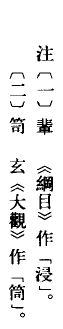
\includegraphics[height=4cm]{image2}
\end{tabular}


\section{Kaiti \chin{楷體}}
\begin{mainrule}
  Please surround the text in kaiti (\chin{楷體}) font as shown on the image with the tags §<k>§ and §</k>§.
\end{mainrule}
\vspace{3mm}

\begin{sampleImageSmall}[\ 3: \, Kaiti \chin{楷體}]{height=10cm}{image3.png}
\hspace{-25mm}
  \begin{typeChinese}
 \f{<h3><k>}\z{玉泉}\f{</k></h3>}\\
 \f{<p><k>}\z{味 甘,平,}\f{</k>}\z{無}\untranscribedText\z{。}\f{<k>}\z{主治}\f{<a>}\z{﹝一﹞}\f{</a>}\z{五}\f{<a>}\z{﹝二﹞}\f{</a>}\z{藏}\untranscribedText\z{柔}\f{<a>}\z{﹝三﹞}\f{</a>}\z{筋}\untranscribedText\z{魄}\f{<a>}\z{﹝四﹞}\f{</a>}\z{,}\\
\someText \f{</p>}
  \end{typeChinese}
  %% shortened the example a bit to make it fit on the page
%% \f{<p><k>}\z{味 甘,平,}\f{</k>}\z{無毒。}\f{<k>}\z{主治}\f{<a>}\z{﹝一﹞}\f{</a>}\z{五}\f{<a>}\z{﹝二﹞}\f{</a>}\z{藏百病,柔}\f{<a>}\z{﹝三﹞}\f{</a>}\z{筋強骨,安魂魄}\f{<a>}\z{﹝四﹞}\f{</a>}\z{,}\\
\end{sampleImageSmall}


\section{Itemized Lists}
\begin{mainrule}
  The book contains also itemized lists as depicted below. Items start
  either with the character "●" (U+25CF) or "○" (U+25CB) or with no character at all.
  Please use the character sequence §" # "§ as a delimiter between items.
\end{mainrule}
\vspace{3mm}

\begin{sampleImageSmall}[\ 4: \, Itemized lists]{height=10cm}{image4.png}
  \begin{typeChinese}
    \f{<h3>}\z{傷寒}\f{</h3>}\\
    \f{<list>}\\
    \z{○麻黃}\f{ # }\z{葛根}\f{ # }\z{○杏人}\f{ # }\z{茈胡}\f{<a>}\z{﹝一﹞}\f{</a>}\f{ # }\z{前胡}\f{ # }\z{●大青}\f{ # }\z{●龍膽}\f{ # }\z{芍<a>﹝二﹞</a>藥}\f{ # }\z{薰草}\\
    \f{ # }\z{升麻}\f{ # }\z{●牡丹}\f{ # }\z{○虎掌}\f{ # }\z{○朮}\f{ # }\z{防己}\f{ # }\z{●石膏}\f{ # }\z{牡蠣}\f{<a>}\z{﹝三﹞}\f{</a>}\f{ # }\z{貝齒}\f{<a>}\z{﹝四﹞}\f{</a> # }\z{鱉甲}\\
    \f{ # }\z{●犀角}\f{ # }\z{●零}\f{<a>}\z{﹝五﹞}\f{</a>}\z{羊角}\f{ # }\z{蔥白}\f{ # }\z{○生薑}\f{ # }\z{●豉}\f{ # }\z{●溺}\f{<a>}\z{﹝六﹞}\f{</a>}\f{ # }\z{●芒消}\\
    \f{</list>}
  \end{typeChinese}
\end{sampleImageSmall}

\end{document}

%%% Local Variables: 
%%% mode: latex
%%% TeX-master: t
%%% End: 
